%File: functional-user.tex
%Date: Sat Oct 19 17:05:21 2013 +0800
%Author: Yikai Zhao <blahgeek@gmail.com>

\subsection{Fetcher}
  As the core component, fetcher is designed to be extremely flexible.
  It will be inherited into various kinds of fetchers to deal with different fetch targets.
  All the fetchers will be executed in a cluster as time based works, just like other web spiders, keeps fetching all the time.

  \begin{figure}[H]
    \centering
    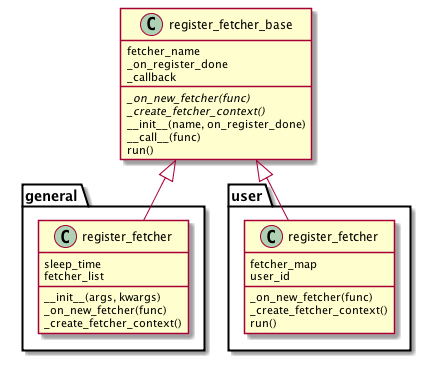
\includegraphics[width=0.8\textwidth]{img/fetcher.png}
    \caption{Fetcher\label{fig:fetcher}}
  \end{figure}

  \subsubsection{Function}
    The fetcher will be assigned to a target website or other kind of source like SNS or RSS feeds.
    Each time called, it will return a list of informations, almost in raw text but with some basic information,
    such as source, origin url, fetched time and so on.

  \subsubsection{Performance}
    Fetcher shall be called at least once per day. For hot resources such as SNS, it's fetcher must have high speed,
    so each time it shall return result in minute level.

  \subsubsection{Input}
    Fetcher don't need input after it's well configured. However, for augmentability reason, a callback function is acceptable.
    The callback function will deal with the result by default.

  \subsubsection{Output}
    Fetcher will return a FetcherContext which wraps the raw information. For default situation, it will be dealed by a Prefilter.

  \begin{figure}[H]
    \centering
    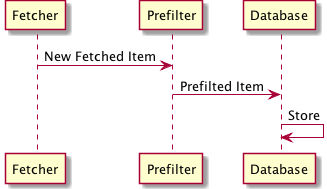
\includegraphics[width=0.6\textwidth]{img/fetch.png}
    \caption{Workflow of Fetcher \label{fig:fetcher}}
  \end{figure}


  Item fetchers simply retrieve items from various information sources,
  adding basic attributes such as ID, description, source URL (if
  available), and then forward items to prefilter for later processing, as illustrated in \figref{fetcher}.

